\providecommand{\main}{..}		% Override relative path to the main file (already set in main file)
\documentclass[../InterneDSLs.tex]{subfiles}
\begin{document}

\chapter{Domänenspezifische Sprachen}\label{SEC:DomainSpecificLanguages}
Domänenspezifische Sprachen sind formale Sprachen, die für eine bestimmte Domäne (Fachbereich) entworfen wurden. Durch diese Modellierung soll eine hohe Spezifität im Bezug auf die Probleme der Domäne gewährleistet werden; und daneben soll nichts anderes ausgedrückt werden können.

Dadurch soll die Sprache für Domänenexperten leicht zu verwenden sein, im Gegensatz zu einer General Purpose Language (siehe~\ref{FIG:DslAdvantages}). Daraus ergibt sich auch, dass der Code besser lesbar ist und weniger Redundanz enthält.

Bei der Entwicklung einer eigenen DSL läuft man aber auch Gefahr, dass diese nur in einer kleinen Nische verwendet wird. Dadurch könnte es auftreten, dass mit vielen DSLs gearbeitet wird, die jeweils nur ihre eigene Domäne abdecken, und man unter Umständen viele Sprachen lernen muss (\ref{FIG:DslDisadvantages}).

\begin{figure}[ht]
\centering
  \begin{subfigure}[c]{0.49\textwidth}
    \begin{itemize}
	  \item Domänenexperten entwickeln
	  \item Lesbarkeit, weniger Redundanz
	  \item Änderung des Ausführungskontextes
    \end{itemize}
    \caption{Vorteile von DSLs}
    \label{FIG:DslAdvantages}
  \end{subfigure}
  \begin{subfigure}[c]{0.49\textwidth}
    \begin{itemize}
	  \item Viele fragmentierte DSLs
	  \item Implementierungsaufwand
	  \item Eigene DSL in kleiner Nische
    \end{itemize}
    \caption{Nachteile von DSLs}
    \label{FIG:DslDisadvantages}
  \end{subfigure}
  \caption{Vor- und Nachteile von DSLs}
  \label{FIG:DslAdvantagesDisadvantages}
\end{figure}


\section{Terminologie}
Im Folgenden werden wichtige Terme über DSLs vorgestellt und erklärt.

\subsection{Domäne}
DSLs werden für einen bestimmten Fachbereich entwickelt, der aus der Informatik selbst kommen kann oder ein fremder sein kann. Beispiele aus der Informatik sind Build-Systeme (Make, Maven, ...) und SQL.

\subsection{Hostsprache}
Eine Hostsprache ist eine General-Purpose Programmiersprache, in die eine interne DSL eingebettet ist.

\subsection{Konkrete Syntax}
Die konkrete Syntax legt durch eine Notation (Schlüsselworte, Symbole, \ldots) fest, wie etwas formuliert werden kann. Dazu können reguläre Ausdrücke oder EBNF-Gram"-ma"-tiken verwendet werden.

\subsection{Abstrakte Syntax}
Die abstrakte Syntax beschreibt die Struktur der Sprache, bzw. was mit ihr formuliert werden kann. Sie kann durch abstrakten Syntax-Baum dargestellt werden.

\subsection{Statische Semantik}
Die statische Semantik sind zusätzliche Einschränkungen für die Wohlgeformtheit von Formulierungen. Konsistenzregeln für abstrakte Syntaxgrafen, die zur Übersetzungszeit geprüft werden könne. Zum Beispiel müssen alle Bezeichner in einem Bereich eindeutig sein-

\subsection{Dynamische Semantik}
Die dynamische Semantik regelt die Bedeutung von Formulierungen, und welches Verhalten von den Formulierungen erzeugt wird. Zum Beispiel wird aus einer Variablendefinition durch den Compiler eine Speicherreservierung.


\section{Probleme und Anwendungsfälle}
DSLs können zum Beispiel für spezielle Unternehmensbereiche (Fakturierung, Lohnabrechnung, ...) oder auch für spezielle Probleme in der Informatik (Datenbankabfragesprachen, Build-Systeme).

Ein Problem kann sein, dass eine DSL nur für eine Nische entwickelt wird und kaum angewandt wird oder nicht rentabel ist. Auch können ähnliche DSLs für denselben Anwendungsfall erstellt worden sein und konkurrieren direkt miteinander. Ein weiteres Problem kann schon beim Design der DSL auftreten, etwa dass die Domäne nicht richtig von der Hostsprache abgegrenzt wurde und mehr als nur Probleme der Hostsprache formuliert werden können.


\section{Interne und Externe Umsetzung}
Domänenspezifische Sprachen lassen sich auf zwei Arten kategorisieren. Man kann sie einerseits in externe und interne DSLs einteilen, zum Anderen kann man sie in ihrer Notation (Abschnitt~\ref{SEC:Notation}) unterscheiden.

\subsection{Externe DSLs}
Externe DSLs sind eigenständige, neu entwickelte Sprachen. Die Konkrete Syntax und Semantik können selbst festgelegt werden und gelten deshalb als mächtiger. Allerdings muss mehr Aufwand für die Erstellung der Tools (Parser, Interpreter/Compiler, \acs{IDE}-Unterstützung) erbracht werden, was für agile Softwareentwicklung nicht optimal ist. Beispiele für externe DSLs sind LaTeX, Awk und SQL.

\subsection{Interne DSLs}
Interne DSLs werden innerhalb einer Hostsprache definiert und können deshalb dessen Tools mitbenutzen, wodurch der Implementierungsaufwand sinkt. Je nach verwendeter Hostsprache ähneln interne DSLs eher einer Bibliothek oder wirken wie eine eigene Sprache. Da der Aufwand bei internen DSLs geringer ist, eignen sie sich besser als Prototyp in agilen Umgebungen.~\cite{butting2018deriving}

Interne DSLs können zum Beispiel als Fluent-\acs{API} umgesetzt werden.


\section{Formulierung innerhalb der Hostsprache}
Interne DSLs kann man, je nach Hostsprache, unterschiedlich umsetzen. Ruby und Scala erlauben mehr Freihet beim Design der Sprache als etwa Java. In Java werden DSLs als (fluent) API umgesetzt, die ähnlich wie Bibliotheken sind, aber in der Formulierung mit Methoden DSLs ähneln. Beispiele sind:
\begin{itemize}
	\item Method Chaining
	\item Object Scoping
	\item Method Sequence
\end{itemize}
Im Folgenden wird kurz auf die Vor- und Nachteile der einzelnen Konstrukte eingegangen.

\subsection{Method Chaining}
Beim Method Chaining werden mehrere Methoden, die ein Objekt manipulieren, direkt nacheinander aufgerufen (z.B. iostream in C++ oder StringBuilder in Java~\ref{LST:StringBuilder}). Nach Fowler ist Method Chaining eine wichtige Methode zur Implementierung von internen DSLs~\cite[S.~373]{Fowler.2010}. Im Prototypen wird deshalb auch direkt Method Chaining angewandt.

Beim Implementieren der Methoden muss darauf geachtet werden, dass sie eine Referenz auf das Objekt selbst zurückgeben, um folgende Aufrufe zu ermöglichen.

\begin{lstlisting}[label=LST:StringBuilder,caption={Method Chaining beim StringBuilder}]
String string = new StringBuilder.append("Hallo ").append("Welt").append('!').toString();
\end{lstlisting}

\subsection{Object Scoping}
Beim Object Scoping werden Methoden in Interfaces bzw. Objekten gekapselt, von denen geerbt werden kann. Dadurch können Methoden auch nur deklariert und später manuell definiert werden; durch die Vererbung kann auch die Wiederholung und optionalen Elemente modelliert werden.

\subsection{Method Sequence}
Die Method Sequence ist eine Aufrufreihenfolge von globalen Funktionen und hat den Nachteil, dass die Funktionen global sind und nicht auf Objekten operieren. Dadurch sind die Daten, nicht wie beim Object Scoping und Method Chaining, nicht gekapselt. Üblicherweise wird von globalen Variablen und Funktionen abgeraten, auch Fowler schätzt das Method Chaining als wenigst nützlich ein~\cite[S. 352]{Fowler.2010}. Auch im Prototypen wird auf Method Sequences verzichtet und stattdessen auf Method Chaining und hauptsächlich Object Scoping gesetzt.

\chapter{Grammatiken}\label{SEC:Grammars}
Programmiersprachen liegen formale Sprachen zugrunde, die in der Chomsky-Hie"-rar"-chie (Abbildung~\ref{fig:chomkskyhierarchie}) gruppiert werden können. Diese formalen Sprachen legen durch Regeln fest, welche Zeichenketten gültig sind und damit zur Sprache gehören. Jede Klasse von Grammatiken beinhaltet auch die Grammatiken tiefer in der Chomsky-Hierarchie. (Überführung ineinander?)

\begin{figure}
\centering
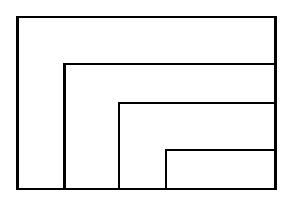
\includegraphics[width=0.5\textwidth]{\main/10_Pictures/Grammatiken}
\caption{Chomsky-Hierarchie}
\label{fig:chomkskyhierarchie}
\end{figure}

\section{Typ-3-Grammatiken}\label{sec:refulaeregrammatik}
Typ-3-Grammatiken entsprechen regulären Grammatiken, die kontextfreie Grammatiken (siehe Abschnitt~\ref{sec:kontextfreiegrammatik}) mit speziellem Einschränkungen sind. Es gibt links- und rechtsreguläre Grammatiken, jedoch ist mit \gqq{regulär} meistens \gqq{rechtsregulär} gemeint. Bei linksregulären Grammatiken sind auf der rechten Seite der Bildungsregeln Nicht-Terminale nur links von den Terminalen erlaubt; bei rechtsregulären Grammatiken dürfen Nicht-Terminale entsprechend nur rechts von den Terminalen stehen. Ein Beispiel für reguläre Grammatiken sind reguläre Ausdrücke.

\section{Typ-2-Grammatiken}\label{sec:kontextfreiegrammatik}
Kontextfreie Grammatiken erlauben auf der rechten Seite der Bildungsregeln eine beliebige Folge von Terminalen und Nicht-Terminalen; auf der linken Seite darf nur ein Nicht-Terminal stehen, das also keinen Kontext hat. Es sind aber mehrere Bildungsregeln für dasselbe Nicht-Terminal erlaubt. Die meisten Programmiersprachen verwenden kontextfreie Grammatiken.\cite{Fowler.2010}

\section{Typ-1-Grammatiken}\label{sec:kontextsensitivegrammatik}
Kontextsensitive Grammatiken erlauben auf der linken Seite der Bildungsregeln links und rechts von dem Nicht-Terminal weitere Terminal- und Nicht-Terminal-Symbole. Dadurch können diese Nicht-Terminale nur im Kontext zu anderen Symbolen auftreten. Auch sollte die rechte Seite der Bildungsregel mindestens gleich lang sein wie die linke. Analog wie bei Regulären Grammatiken (siehe Abschnitt~\ref{sec:refulaeregrammatik}) gibt es links-kontextsensitive und rechts-kontextsensitive Grammatiken, bei denen links respektive rechts vom Nicht-Terminal-Symbol weitere Symbole stehen.

\section{Typ-0-Grammatiken}\label{sec:beliebigegrammatik}
Beliebige formale Grammatik haben keine Einschränkungen, außer dass bei keiner Bildungsregel auf der linke Seite die leere Zeichenkette stehen darf. Der einzige Unterschied zu kontextsensitiven Grammatiken ist der, dass das Nicht-Terminal-Symbol neben einem Kontext auf der rechten Seite auch der leere String werden darf.


\section{Notation}\label{SEC:Notation}
DSLs können auch in der Art der Notation unterschieden werden, es gibt grafische und textuelle DSLs. Ein Beispiel für eine grafische DSL ist UML, textuelle DSLs sind zum Beispiel HTML oder LaTeX. Fowler stellt auch Workbenches vor.\cite[S. 22ff]{Fowler.2010}

\subsection{EBNF}
Die erweiterte Backus-Naur-Form ist eine Erweiterung der Backus-Naur-Form, um die Syntax von kontextfreien Grammatiken zu notieren. Sie wurde ursprünglich für die Syntax von Pascal eingeführt. Es gibt verschiedene Varianten der Notation (z.B.~\cite{wirthsyntaxnotation.wikipedia} und \cite{ebnfnotations.jinks}) und ist inzwischen ein ISO-Standard\\cite{scowen1996international}, der ebenfalls einen neuen Dialekt einführt.

Die EBNF vereinfacht das Ausdrücken von optionalen Elementen und Wiederholungen, wodurch keine zusätzlichen Regeln benötigt werden.

\subsection{Grafisch}
Es gibt auch grafische Notationen für DSLs, etwas das Eclipse Modeling Framework\footnote{\url{http://www.eclipse.org/emf/}}, das sich an der Notation für Klassen von UML anlehnt.

Wegen der weiten Verbreitung der EBNF und einfachen Implementierbarkeit einer Textverarbeitung im Vergleich zu einem grafischen Editor wird in dieser Arbeit die EBNF zur Notation verwendet.

\end{document}
